%
% File acl2019.tex
%
%% Based on the style files for ACL 2018, NAACL 2018/19, which were
%% Based on the style files for ACL-2015, with some improvements
%%  taken from the NAACL-2016 style
%% Based on the style files for ACL-2014, which were, in turn,
%% based on ACL-2013, ACL-2012, ACL-2011, ACL-2010, ACL-IJCNLP-2009,
%% EACL-2009, IJCNLP-2008...
%% Based on the style files for EACL 2006 by 
%%e.agirre@ehu.es or Sergi.Balari@uab.es
%% and that of ACL 08 by Joakim Nivre and Noah Smith

\documentclass[11pt,a4paper]{article}
\usepackage{authblk}
\usepackage[hyperref]{acl2019}
\usepackage{times}
\usepackage{IEEEtrantools}
\usepackage{latexsym}
\usepackage{amsmath}
\usepackage{mathtools}

\usepackage{multirow}
\usepackage{algorithm}
\usepackage{graphicx}
\usepackage{booktabs}
\usepackage[inline]{enumitem}
\usepackage{bm}
\usepackage{caption}


\usepackage{url}

\aclfinalcopy % Uncomment this line for the final submission
\def\aclpaperid{890} %  Enter the acl Paper ID here

%\setlength\titlebox{5cm}
% You can expand the titlebox if you need extra space
% to show all the authors. Please do not make the titlebox
% smaller than 5cm (the original size); we will check this
% in the camera-ready version and ask you to change it back.

\newcommand\BibTeX{B\textsc{ib}\TeX}

%\title{Joint Entity Relation Extraction with Graph Convolutional Network}
\title{Joint Type Inference on Entities and Relations via Graph Convolutional Networks}
%\title{End-to-End Neural Relation Extraction with Joint Type Inference}
%\title{Joint Type Inference for Extracting Entities and Relations}

%\author{First Author \\
%  Affiliation / Address line 1 \\
%  Affiliation / Address line 2 \\
%  Affiliation / Address line 3 \\
%  \texttt{email@domain} \\\And
%  Second Author \\
%  Affiliation / Address line 1 \\
%  Affiliation / Address line 2 \\
%  Affiliation / Address line 3 \\
%  \texttt{email@domain} \\}

\author[1, \thanks{\ \ \ Work done while this author was an intern at Microsoft Research Asia.}]{\bf Changzhi Sun  }
\author[2]{\bf Yeyun Gong}
\author[1, 3]{\bf Yuanbin Wu}
\author[2]{\bf Ming Gong}
\author[2]{\bf Daxing Jiang}
\author[1]{\\ \bf Man Lan}
\author[1]{\bf Shiliang Sun}
\author[2]{\bf Nan Duan}
\affil[1]{Department of Computer Science and Technology, East China Normal University}
\affil[2]{Microsoft Research Asia}
\affil[3]{State Key Laboratory of Cognitive Intelligence, iFLYTEK}
\affil[  ]{\tt \{changzhisun\}@stu.ecnu.edu.cn \{ybwu,mlan,slsun\}@cs.ecnu.edu.cn}
%\affil[ ]{\tt \{ybwu,mlan,slsun\}@cs.ecnu.edu.cn}
\affil[  ]{\tt \{yegong, nanduan, migon, djiang\}@microsoft.com}


\begin{document}
\maketitle
\begin{abstract}
  We develop a new paradigm for the task of joint entity relation extraction.
  It first identifies entity spans,
  then performs a joint inference on entity types and relation types.
  To tackle the joint type inference task,
  we propose a novel graph convolutional network (GCN)
  running on an entity-relation bipartite graph.
  By introducing a binary relation classification task,
  we are able to utilize the structure of entity-relation  bipartite graph in a more efficient and interpretable way.
  Experiments on ACE05 show that our
  model outperforms existing joint models in entity performance
  and is competitive with the state-of-the-art in relation performance.
\end{abstract}

\section{Introduction}
Extracting entities and relations from plain texts
is an important and challenging task in natural language processing.
Given a sentence,
the task aims to detect text spans with specific types (\emph{entities})
and semantic relations among those text spans (\emph{relations}).
For example, in the Figure \ref{fig:example},
``Toefting'' is a person entity (\texttt{PER}), 
``teammates'' is a person entity (\texttt{PER}), 
and the two entities have a Person-Social relation (\texttt{PER-SOC}).

To tackle the task of entity relation extraction,
various methods have been proposed,
which can be divided into two categories: pipeline models and joint models.
Pipeline models extract entities and relations in two stages:
entities are first extracted by an entity model,
and then these extracted entities are used as the inputs of a relation model.
Pipeline models often ignore interactions between the two models and 
they suffer from error propagation. Joint models integrate information between entities and relations
into a single model with the joint training,
and have achieved better results than the pipeline models.
In this paper, we focus on joint models.
\begin{figure}[t]
    \begin{center}
        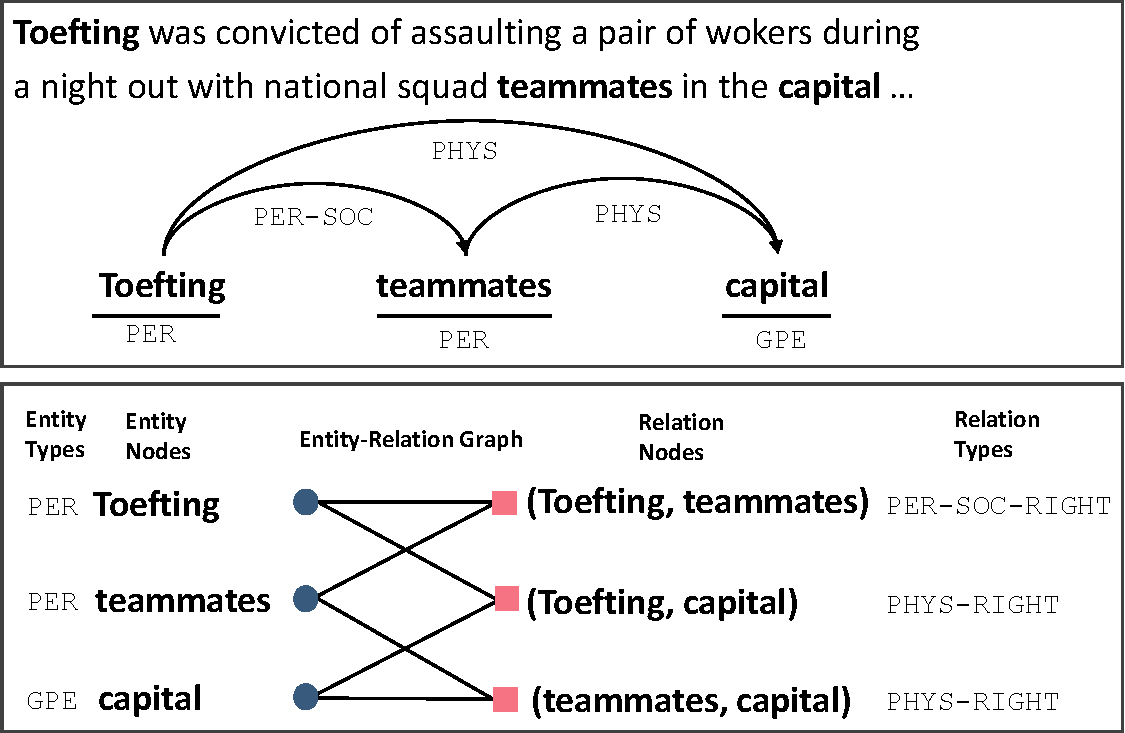
\includegraphics[width=3.0in]{../images/fig-example.pdf}
    \end{center}
    \caption{An example from ACE05. The first part contains annotations
    and the second part is the entity-relation graph of the sentence used in GCN.}
    \label{fig:example}
\end{figure}



More and more joint methods have been applied to this task. 
Among them,
\citet{miwa-bansal:2016:P16-1,katiyar-cardie:2017:Long}
identify the entity with a sequence labelling model,
and identify the relation type with a multi-class classifier.
These joint methods do joint learning through sharing parameters 
and they have no explicit interaction in type inference.
In addition,
some complex joint decoding algorithms 
(e.g., simultaneously decoding entities and relations in beam search) 
have been carefully investigated, including~\citet{li-ji:2014:P14-1,
zhang-zhang-fu:2017:EMNLP2017,zheng-EtAl:2017:Long,wang2018joint}.
They jointly handle span detection and type inference to achieve more interactions.

By inspecting the performance of existing models \cite{D18-1249} on ACE05, 
we find that,
for many entities, their spans are correctly identified,
but their entity types are wrong.
In particular,
the F1 of extracting typed entities is about 83\%,
while the F1 of extracting entity spans is about 90\%.
Thus, if we have a better type inference model,
we may get a better joint extraction performance.
At the same time,
we observe that a joint inference on entity and relation types 
could be potentially better than predicting them independently.
For example, in Figure~\ref{fig:example},
the~\texttt{PER-SOC} relation suggests that the type of  ``Toefting'' might be~\texttt{PER}, and vice versa.
Moreover the \texttt{PER} (``Toefting'') and the relation~\texttt{PER-SOC} could
benefit from other relations such as \texttt{PHYS}.

In this paper,
we define joint entity relation extraction into two sub-tasks:
entity span detection and entity relation type deduction.
For entity span detection,
we treat it as a sequence labeling problem.
For joint type inference,
we propose a novel and concise joint model based on graph convolutional networks (GCNs) \cite{kipf2017semi}.
The two sub-models are trained jointly.
Specifically,
given all detected entity spans in a sentence,
we define an entity-relation bipartite graph.
For each entity span,
we assign an entity node.
For each entity-entity pair,
we assign a relation node.
Edges connect relation nodes and their entity nodes
(last part of Figure \ref{fig:example}).
With efficient graph convolution operations,
we can learn representations for entity nodes and relation nodes
by recursively aggregating information from their neighborhood
over the bipartite graph.
It helps us to concisely capture information among entities and relations.
For example, in Figure \ref{fig:example},
to predict the \texttt{PER} (``Toefting''),
our joint model can pool the information of \texttt{PER-SOC}, \texttt{PHYS},
\texttt{PER} (``teammates'') and \texttt{GPE} (captital).


To further utilize the structure of the graph,
we also propose assigning different weights on graph edges.
In particular,
we introduce a binary relation classification task,
which is to determine whether the two entities form a valid relation.
Different from previous GCN-based models \cite{shang2018end,zhang2018graph},
the adjacency matrix of graph is based on the output of binary relation classification,
which makes the proposed adjacency matrix  more explanatory.
%We compile the proposed joint model with a
%neural network-based model which uses recurrent neural network (RNN) and convolutional neural network (CNN)  similar to~\cite{D18-1249}.
%On  ACE05 dataset,
%we show that the proposed joint model
%is competitive with the state-of-the-art.
To summarize,
the main contributions of this work are
\footnote{ Our implementation is available at  \url{https://github.com/changzhisun/AntNRE}.}
\begin{itemize}[leftmargin=*]
    %\item We define the task of joint entity extraction including entity span detection and entity relation type deduction,
    %which makes it easier to consider the interactions on entity types and relation types jointly. 
    \item We present a novel and concise joint model to handle the joint type inference problem based on graph convolutional network (GCN).
    \item We introduce a binary relation classification task to explore the structure of entity-relation bipartite graph in a more efficient and interpretable way.
    \item We show that the proposed joint model on ACE05
    achieves best entity performance, and is competitive with the state-of-the-art in relation performance.
    
\end{itemize}

\section{Background of GCN}  \label{section:gcn}
In this section, we briefly describe graph convolutional networks (GCNs).
Given a graph with $n$ nodes, 
the goal of GCNs is to learn structure-aware node representations on the graph which takes as inputs:
\begin{itemize}[leftmargin=*, itemindent=1pc]
    \item an $n \times d$ input node embedding matrix $\mathbf{H}$, where $n$ is the number of nodes and $d$ is the dimension of input node embedding;
    \item an $n \times n$ matrix representation of the graph structure such as the adjacency matrix $\mathbf{A}$  (or some function thereof) \footnote{In order to incorporate self-information,
we add a self-loop to each node, where $\mathbf{A}_{ii} = 1.0$ for each node $i$.}.
\end{itemize}

In an L-layer GCNs, every layer can be written as a non-linear function
\begin{IEEEeqnarray}{l}
  \mathbf{H}^{(l+1)} = \sigma (\hat{\mathbf{A}} \mathbf{H}^{(l)} \mathbf{W}^{(l)})
\end{IEEEeqnarray}
with $\mathbf{H}^{(0)} = \mathbf{H}$, 
where $\hat{\mathbf{A}} = \mathbf{D}^{-\frac{1}{2}} \mathbf{A} \mathbf{D}^{-\frac{1}{2}}$  is the normalized symmetric adjacency matrix
and $\mathbf{W}^{(l)}$ is a parameter matrix for the $l$-th GCN layer.
$\mathbf{D}$ is the diagonal node degree matrix, where $\mathbf{D}_{ii} = \sum_j \mathbf{A}_{ij}$.
$\sigma$ is a non-linear activation function like  $\mathrm{ReLU}$.
Finally, we can obtain a node-level output $\mathbf{Z} = \mathbf{H}^{(L)}$,
which is an $n \times d$ feature matrix.

\section{Approach}

We define the joint entity relation extraction task.
Given a sentence
$s = w_1, \dots w_{|s|}$ ($w_i$ is a word), 
the task is to extract a set of entity spans $\mathcal{E}$ with specific types
and a set of relations $\mathcal{R}$.
An entity span $e \in \mathcal{E}$ is a sequence of words
labeling with an entity type $y$ 
(e.g., person (\texttt{PER}), organization (\texttt{ORG})).
%To extract entities, we can first find the start and end positions of them,
%then determine their entity types.
%Formally, we define the task of entity span detection.
%It focus on locating boundaries of entities.
A relation $r$ is a quintet $(e_1, y_1, e_2, y_2, l)$, 
where $e_1$ and $e_2$ are two entity spans with specific types $y_1$ and $y_2$.
$l$ is a relation type describing the semantic relation between two entities. 
(e.g., organization affiliation relation (\texttt{ORG-AFF})).
Let $\mathcal{T}_e$, $\mathcal{T}_r$ be the set of possible entity types and relation types respectively.

In this work, we decompose the joint entity relation extraction task into two parts, namely,
entity span detection and entity relation type deduction.
We first treat entity span detection as a sequence labelling task (Section  \ref{section:ent_span}),
and then construct an entity-relation bipartite graph (Section \ref{section:ent-rel-graph}) to perform joint type inference on entity nodes and relation nodes (Section \ref{section:joint-type-inference}).
All sub-models  share parameters and are trained jointly.
Different from existing joint learning algorithms \cite{D18-1249,zhang-zhang-fu:2017:EMNLP2017,katiyar-cardie:2017:Long,miwa-bansal:2016:P16-1},
we propose a concise joint model to perform joint type inference
on entities and relations based on GCNs.
It considers interactions among multiple entity types and relation types
simultaneously in a sentence.
%\begin{figure*} 
%    \begin{center}
%        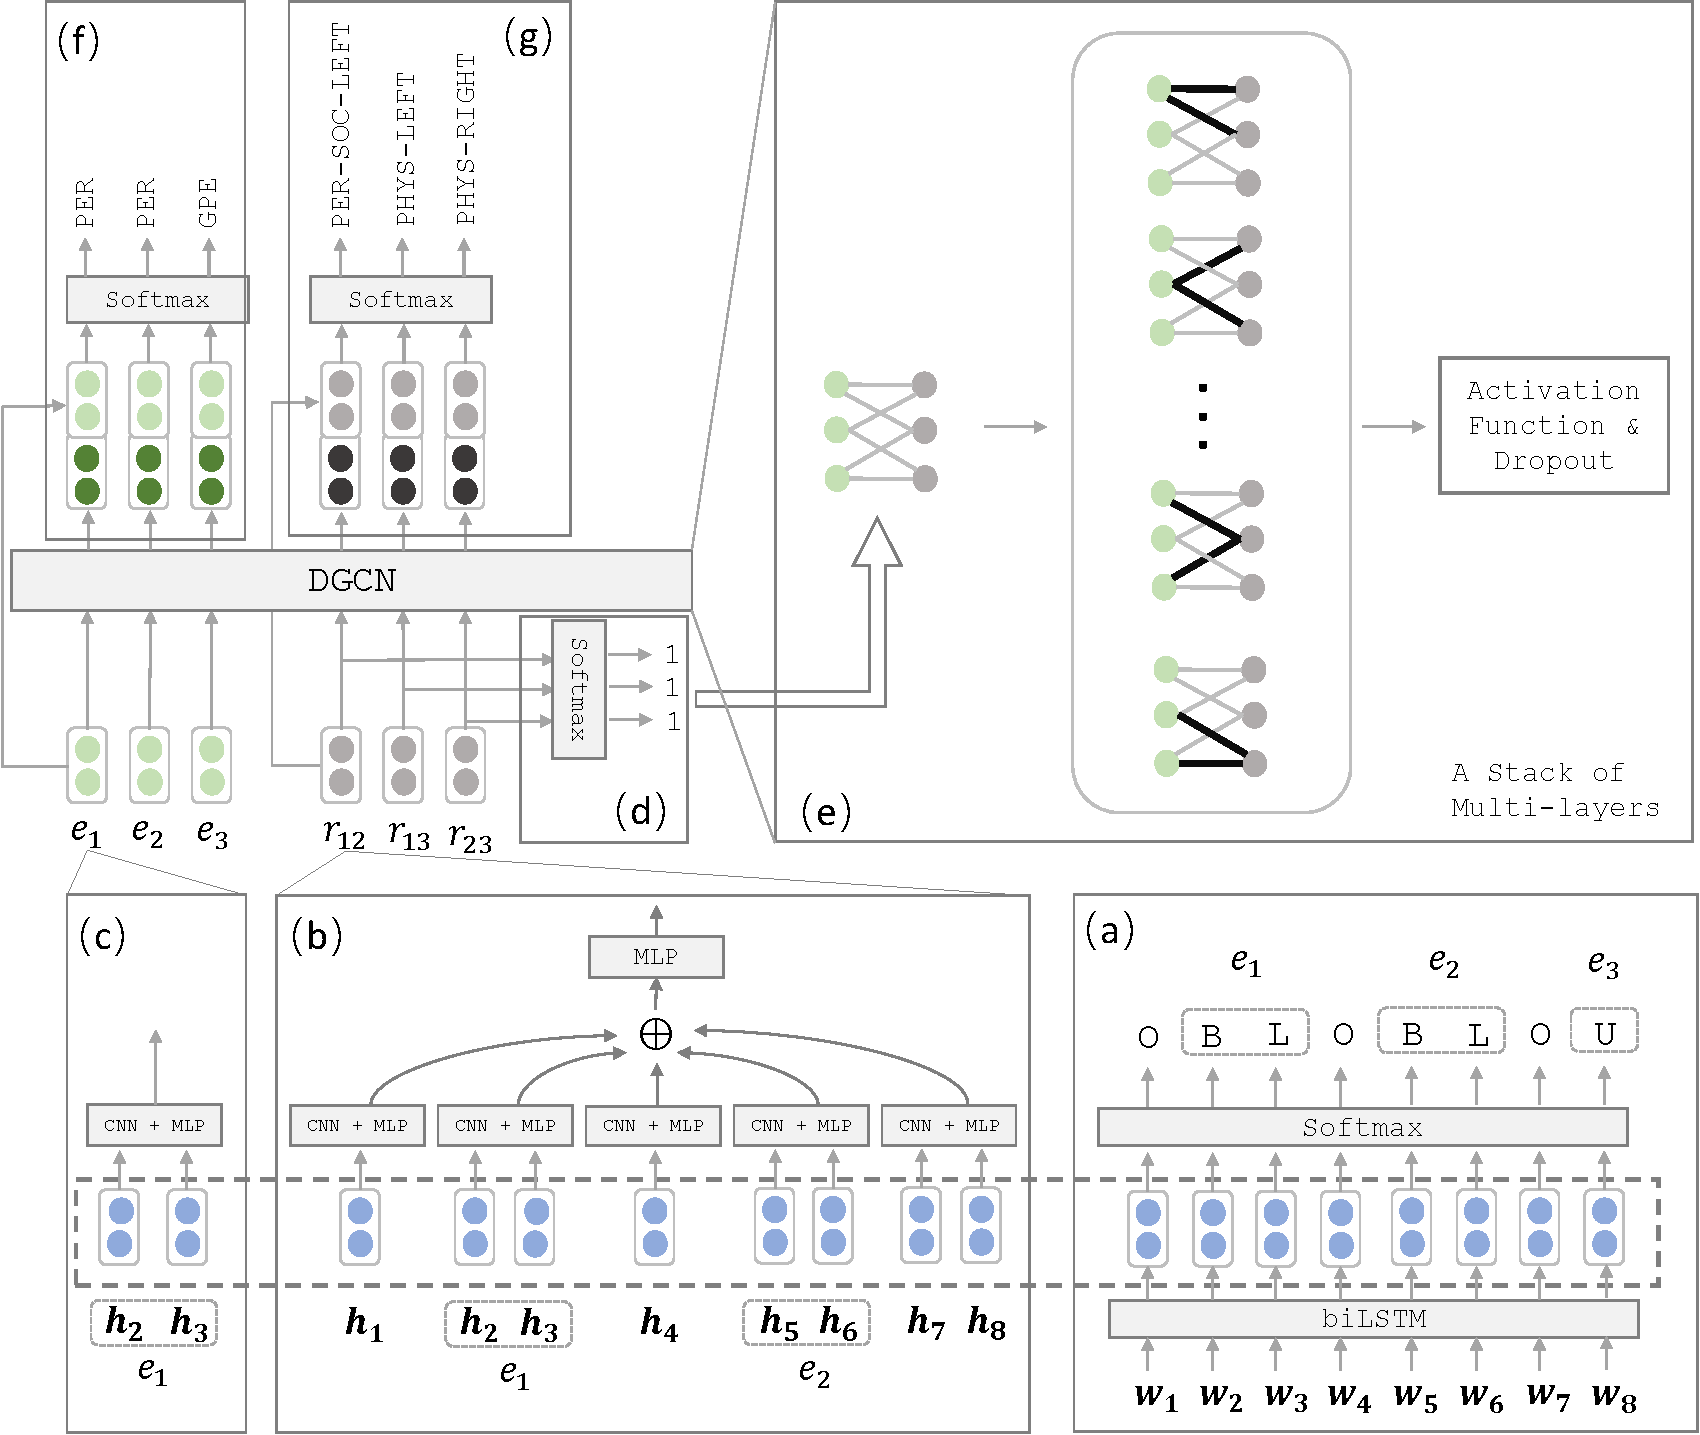
\includegraphics[width=5.0in]{../images/fig-model.pdf}
%    \end{center}
%    \caption{Our network structure for joint entity and relation extraction.}
%    \label{fig:net}
%\end{figure*}
\subsection{Entity Span Detection} \label{section:ent_span}
To extract entity spans from a sentence (Figure \ref{fig:ent-span}),
we adopt the \texttt{BILOU} sequence tagging scheme: 
\texttt{B}, \texttt{I}, \texttt{L} and \texttt{O} denote the begin,
inside, last and outside of a target span,
\texttt{U} denotes a single word span.
For example, for a person (\texttt{PER}) entity ``Patrick McDowell'', 
we assign \texttt{B} to ``Patrick'' and \texttt{L} to ``McDowell''.

Given an input sentence $s$,
we use a bidirectional long short term memory (biLSTM) network  \cite{DBLP:journals/neco/HochreiterS97} with parameter $\theta_\mathrm{seq}$
to incorporate information from both forward and backward directions of $s$.
\begin{IEEEeqnarray}{l}
    \mathbf{h}_i = \mathrm{biLSTM}(\mathbf{x}_i; \theta_\mathrm{seq}), \label{eq:bilstm}
\end{IEEEeqnarray}
where $\mathbf{h}_i$ is the concatenation of a forward and a backward LSTM's hidden states at position $i$,
and $\mathbf{x}_i$ is the word representation of $w_i$
which contains pre-trained embeddings and
character-based word representations
generated by running a CNN on the character sequences of $w_i$.
Then, we employ a softmax output layer to predict $w_i$'s tag $\hat{t}_i$,
\begin{IEEEeqnarray*}{c}
    \label{eq:ent_span_prob}
    P(\hat{t}_i|s)=\mathrm{Softmax}(\mathbf{W}_\mathrm{span}\mathbf{h}_i),
\end{IEEEeqnarray*}
where $\mathbf{W}_\mathrm{span}$ is the parameter. 
Given an input sentence $s$ and its gold tag sequence $\mathbf{t} = t_1, \dots, t_{|s|}$,
the training objective is to minimize
\footnote{We have also tried biLSTM-CRF \cite{DBLP:journals/corr/HuangXY15} 
as an advanced sequence labelling model, 
but performances are nearly the same in our experiments.
}
\begin{IEEEeqnarray}{c}
    \mathcal{L}_\mathrm{span} = 
    -\frac{1}{|s|} \sum_{i=1}^{|s|} \log P(\hat{t}_i = t_i|s).
    \label{eq:loss_seq}
\end{IEEEeqnarray}

\begin{figure} 
    \begin{center}
        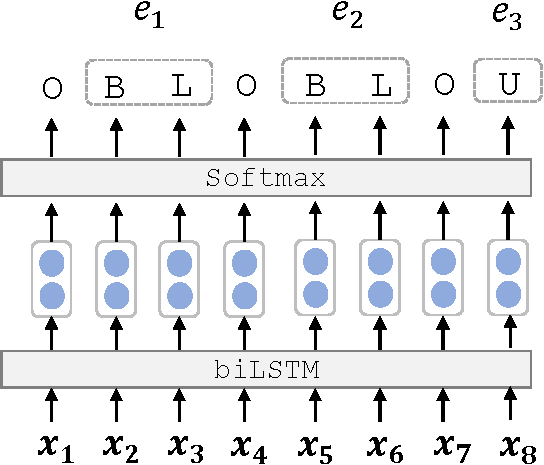
\includegraphics[width=2.5in]{../images/ent-span.pdf}
    \end{center}
    \caption{The biLSTM model for entity span detection.}
    \label{fig:ent-span}
\end{figure}

\subsection{Entity-Relation Bipartite Graph} \label{section:ent-rel-graph}

Given a set of detected entity spans $\hat{\mathcal{E}}$
(obtained from the entity span tag sequence $\hat{\mathbf{t}}$),
we consider all entity span pairs in $\hat{\mathcal{E}}$ as candidate relations
\footnote{The first entity span is always on the left side of the second entity span of each candidate relation, and we use in total $2\mathcal{T}_r+1$ relation types in order to consider both directions.
The additional type is the \texttt{None}  which means no relation between entity span pair.}.
Then we build a heterogeneous undirected bipartite graph $\mathcal{G}^s$ which contains entity nodes and relation nodes in a sentence $s$.
In the graph $\mathcal{G}^s$, interactions  on  multiple  entity types and relation types can be explicitly modeled. 
The number of nodes $n$ in the graph $\mathcal{G}^s$ is the number of entity spans
$|\hat{{\mathcal{E}}}|$ plus the number of all candidate relations $\frac{|\hat{{\mathcal{E}}}| (|\hat{{\mathcal{E}}}| - 1)}{2}$.
We have an initial input node embedding matrix $\mathbf{H}$.
For a relation $r_{12}$ and its two entities $e_1, e_2$,
we use $\mathbf{H}_{r_{12}}$ to denote relation embedding of $r_{12}$,
and use
$\mathbf{H}_{e_1}$,$\mathbf{H}_{e_2}$ to denote entity embedding of $e_1, e_2$ respectively.


\begin{figure*} 
    \begin{center}
        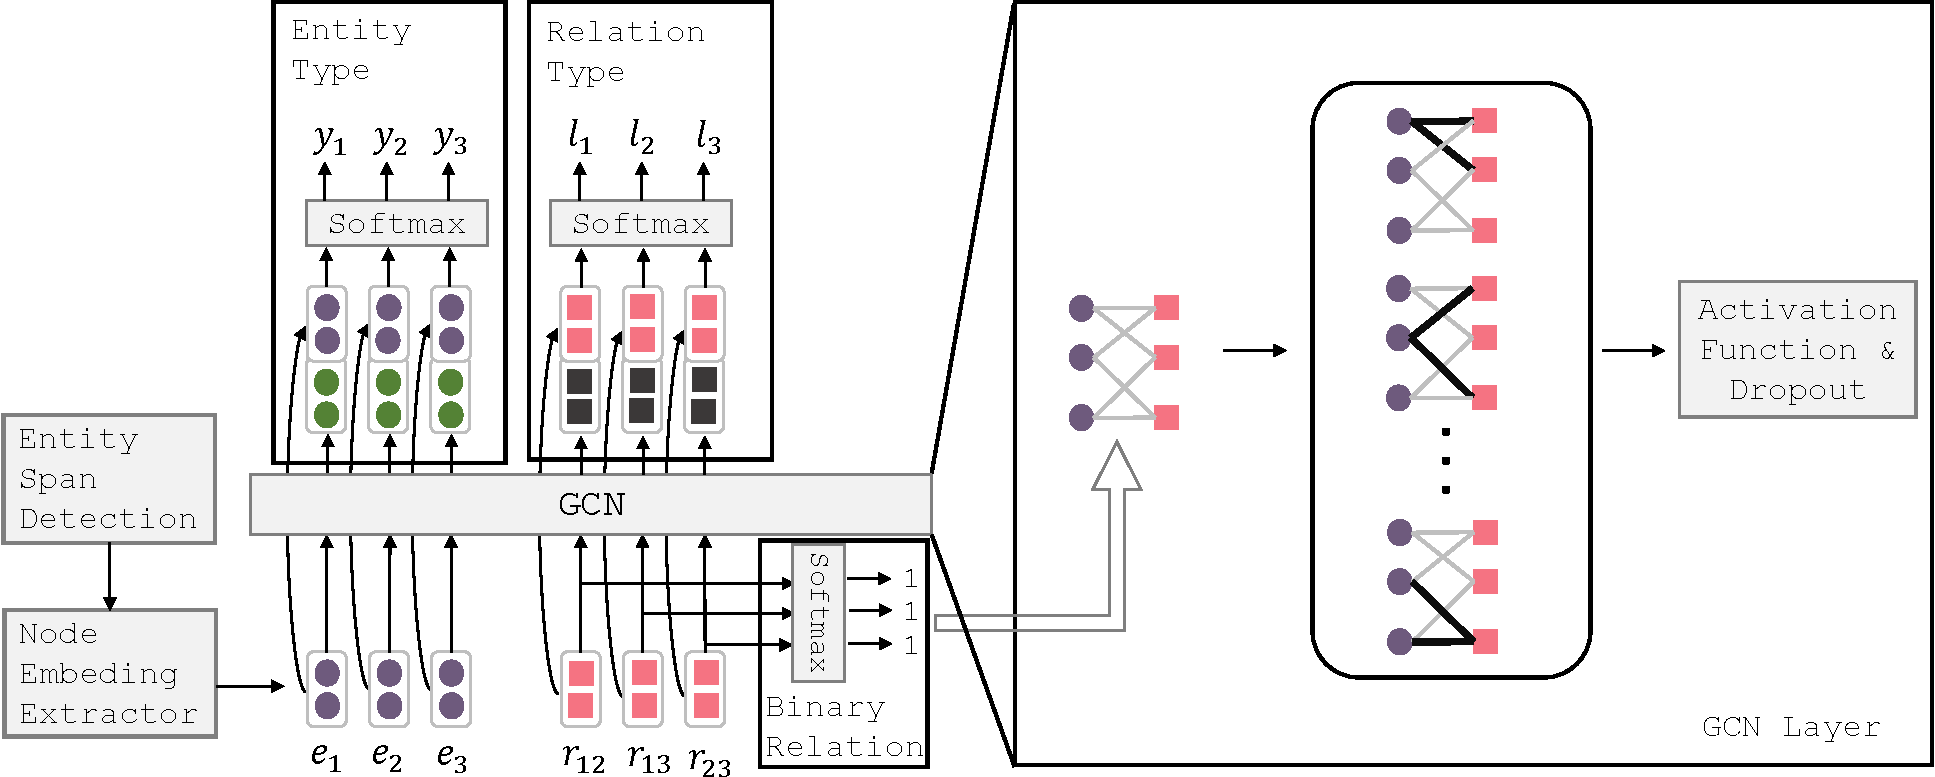
\includegraphics[width=6.0in]{../images/gcn.pdf}
    \end{center}
    \caption{Our network structure for the joint entity and relation extraction based on GCN. The node embedding extractor computes $\mathbf{H}_e$ and $\mathbf{H}_r$.}
    \label{fig:gcn}
\end{figure*}


Next, we build edges between entity nodes and relation nodes.
For graph edges,
we connect every relation node to its two entity nodes
instead of directly connecting any entity (relation) nodes.
Thus we focus on the bipartite graph.
The reasons are two folds. a) We do not think 
that all the remaining entities in the sentence are helpful.
Relation nodes are bridges between entity nodes and vice versa.
b) GCN is not suitable for fully-connected graphs  
because GCN reduce to rather trivial operations on fully-connected graphs.
It means that,
for an entity node $e$, the only way to observe other entities 
is through relations which $e$ takes part in.
For example, given a relation node $r_{12}$ and its two entity nodes $e_1, e_2$,
we add two edges. One is the edge between $e_1$ and $r_{12}$,
and another is the edge between $e_2$ and $r_{12}$.
We refer to it as \textbf{static} graph.

In order to further utilize the structure  of  the  graph (some kind of prior knowledge)
instead of using a static graph, 
we also investigate the \textbf{dynamic} graph for pruning redundant edges.
A key intuition is that if two entities hold a relation,
we could add two edges between the relation node and two entity nodes.
Conversely, if two entities have no relation,
we keep two entity nodes and the relation node separately.
To this end, we introduce the \textbf{binary relation classification} task.
It aims to predict whether a certain relation exists 
between an entity span pair (ignoring specific relation types).
We build a binary relation model which predicts a label in $\{0, 1\}$ 
to indicate the existence of a candidate relation 
based on relation node embedding.
Given a relation node $r_{ij}$ in a sentence $s$,
to get the posterior of the binary relation label $\hat{b}$,
we apply softmax layer on the relation node embedding $\mathbf{H}_{r_{ij}}$,
\begin{IEEEeqnarray*}{c}
    \label{eq:bin_rel_prob}
    P(\hat{b}| r_{ij}, s)=\mathrm{Softmax}(\mathbf{W}_\mathrm{bin}\mathbf{H}_{r_{ij}}),
\end{IEEEeqnarray*}
where $\mathbf{W}_\mathrm{bin}$ is the parameter.
The training objective is to minimize
\begin{IEEEeqnarray}{c}
    \mathcal{L}_{\mathrm{bin}} = - 
    \sum_{r_{ij}} 
    \frac{\log P(\hat{b} = b |r_{ij}, s)}
    {\mathrm{\#\ candidate\ relations}\ r_{ij}},
    \label{eq:loss_bin}
\end{IEEEeqnarray}
where true binary annotations $b$ are transformed from the original typed relation labels. Formally, the adjacency matrix $\mathbf{A}$  is defined as 
\begin{itemize}[leftmargin=*, itemindent=1pc]
    \item if $P(\hat{b} = 1 | r_{ij}, s) > 0.5$, we set the value of $\mathbf{A}$ between entity nodes $e_i, e_j$ and relation node $r_{ij}$ to 1.0,
    \item the diagonal elements of $\mathbf{A}$ are set to 1.0,
    \item while others are set to 0.0.
\end{itemize}

To compare with \textbf{hard} binary value $\mathbf{A}$,
we also try the \textbf{soft} value $\mathbf{A}$ in experiments.
It means that we set the value of $\mathbf{A}$ between entity nodes $e_i, e_j$ and relation node $r_{ij}$ 
to the probability $P(\hat{b} = 1 | r_{ij}, s)$ except for the diagonal elements (they are set to 1.0).

Here, we introduce how to compute two types of contextualized node embedding in the graph $\mathcal{G}^s$:
entity node embedding and relation node embedding.

\vspace{0.5em}
\noindent
\textbf{Entity Node Embedding}  
Given an entity span $e \in \hat{\mathcal{E}}$,
for each word $w_i \in e$,
we first collect $w_i$'s biLSTM hidden vector $\mathbf{h}_i$ from entity span model.
Then, we use a CNN (a single convolution layer with a max-pooling layer) with a multi-layer perceptron (MLP)
on vectors $\{\mathbf{h}_i | w_i \in e \}$
to obtain the resulting $d$-dimensional entity span node embedding $\mathbf{H}_{e}$ ($\mathbf{H}$ is a matrix mentioned before in Section \ref{section:gcn}),
as shown in the left part of Figure \ref{fig:node}.

\vspace{0.5em}
\noindent
\textbf{Relation Node Embedding}
Given a candidate relation $r_{12}$, 
we extract two types of features,
namely, features regarding words in $e_1, e_2$ 
and features regarding contexts of the entity span pair $(e_1, e_2)$.
For features on words in $e_1, e_2$,
we simply use entity node  embedding $\mathbf{H}_{e_1}$ and $\mathbf{H}_{e_2}$.
For context features of the entity span pair $(e_1, e_2)$,
we build three feature vectors by looking at words
between $e_1$ and $e_2$, words on the left of the
pair and words on the right of the pair.
Similarly, we build three features by running another CNN with an MLP.
Finally, the five feature vectors are concatenated to a single vector.
To get $d$-dimensional relation node embedding $\mathbf{H}_{r_{12}}$, 
we apply an MLP on the single vector,
as shown in the right part of Figure \ref{fig:node}.
\begin{figure} 
    \begin{center}
        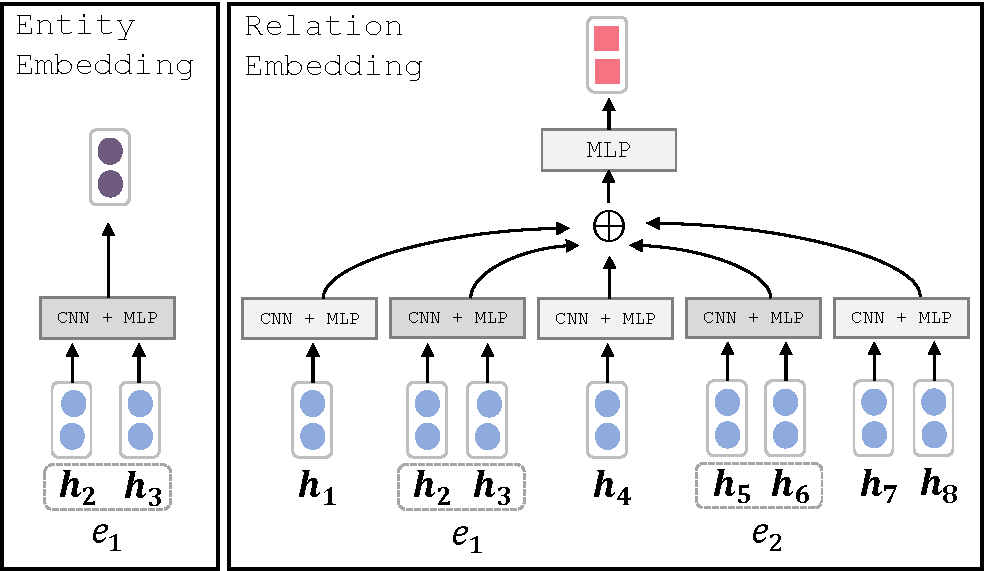
\includegraphics[width=3.0in]{../images/node-repr.pdf}
    \end{center}
    \caption{Our node embedding extractor.}
    \label{fig:node}
\end{figure}
\subsection{Joint Type Inference} \label{section:joint-type-inference}

After building the entity-relation bipartite graph,
we feed the graph into a multi-layer GCNs 
to obtain the node-level output $\mathbf{Z}$.
For each row in $\mathbf{Z}$ (entity or relation node representation), 
it can gather and summarize information from other
nodes in the graph $\mathcal{G}^s$ although
there is no direct entity-entity or relation-relation edges in the graph.
Then the final node representation $\mathbf{F}$ of graph $\mathcal{G}^s$ is concatenated by 
the input node embedding $\mathbf{H}$ and the node-level output $\mathbf{Z}$ ($\mathbf{H}, \mathbf{Z}$ and $\mathbf{F}$ are matrices).

Given an entity node $e_i$ and a relation node $r_{ij}$,
to predict the corresponding node types,
we pass the resulted node representation  into two fully connected layer 
with a softmax function, respectively,
\begin{IEEEeqnarray*}{c}
    \label{eq:ent_prob}
    P(\hat{y}| e_i, s)=\mathrm{Softmax}(\mathbf{W}_\mathrm{ent}\mathbf{F}_{e_i}),
\end{IEEEeqnarray*}
\begin{IEEEeqnarray*}{c}
    \label{eq:rel_prob}
    P(\hat{l}| r_{ij}, s)=\mathrm{Softmax}(\mathbf{W}_\mathrm{rel}\mathbf{F}_{r_{ij}}),
\end{IEEEeqnarray*}
where $\mathbf{W}_\mathrm{ent}$, $\mathbf{W}_\mathrm{rel}$ are parameters.
And the training objective is to minimize
\begin{IEEEeqnarray}{c}
    \mathcal{L}_{\mathrm{ent}} = - \frac{1}{|\hat{\mathcal{E}}|}
    \sum_{e_i \in \hat{\mathcal{E}}} 
    \log P(\hat{y} = y |e_i, s),
    \label{eq:loss_ent}
\end{IEEEeqnarray}

\begin{IEEEeqnarray}{c}
    \mathcal{L}_{\mathrm{rel}} = - 
    \sum_{r_{ij}} 
    \frac{\log P(\hat{l} = l |r_{ij}, s)}
    {\mathrm{\#\ candidate\ relations}\ r_{ij}},
    \label{eq:loss_rel}
\end{IEEEeqnarray}
where the true label $y, l$ can be read from annotations,
as shown in Figure \ref{fig:gcn}.

\subsection{Training}
To train the joint  model,
we optimize the combined objective function 
$\mathcal{L} = \mathcal{L}_\mathrm{span} + \mathcal{L}_\mathrm{bin} + \mathcal{L}_\mathrm{ent} +  \mathcal{L}_\mathrm{rel} $,
where the training is accomplished by the shared parameters.
We employ the scheduled sampling strategy
\cite{bengio2015scheduled}
in the entity model similar to
\cite{miwa-bansal:2016:P16-1}.
We optimize our model using Adadelta \cite{zeiler2012adadelta}
with gradient clipping.
The network is regularized with dropout.
Within a fixed number of epochs,
we select the model according to the best relation performance
on development sets\footnote{
Our word embeddings is initialized
with 100-dimensional glove \cite{pennington-socher-manning:2014:EMNLP2014} word embeddings.
The dimensionality of the hidden units and node embedding are set to 128.
For all CNN in our network, 
the kernel sizes are 2 and 3, 
and the output channels are 25.}.
\section{Experiments}
We conduct experiments on \textbf{ACE05} dataset,
which is a standard corpus for the entity relation extraction task.
It includes 7 entity types and 6 relation types between entities.
We use the same data split of ACE05 documents as previous work
(351 training, 80 development and 80 testing) \cite{miwa-bansal:2016:P16-1}.

We evaluate the performances using precision (P), recall
(R) and F1 scores following \cite{miwa-bansal:2016:P16-1,D18-1249}.
Specifically, an output entity $(e, y)$ is correct
if its type $y$ and the region of its head $e$ are correct, and an output
relation $r$ is correct if its $(e_1, y_1, e_2, y_2, l)$ are correct ( i.e., “exact match”).

In this paper, the default setting ``GCN'' is the 1-layer GCN-based joint model 
with the dynamic hard adjacency matrix, which achieves the best relation performance on ACE05 dataset.
\subsection{End-to-End Results on ACE05}



First, we compare proposed models with previous work in Table~\ref{tab:res-baseline-ace}.
In general,
our ``GCN''  achieves the best entity performance 84.2 percent
comparing with existing joint models.
For relation performance,
our ``GCN''  significantly outperforms all joint models 
except for \cite{D18-1249} which uses more complex joint decoder.
Comparing with our basic neural network ``NN'',
our ``GCN'' has large improvement both on entities and relations.
Those observations demonstrate the effectiveness of our ``GCN''  
for capturing information on multiple entity types and relation types from a sentence.

Compared to the state-of-the-art method which adopts minimum risk training \cite{D18-1249},
our ``GCN''   has better entity performance and comparable relation performance.
Different from existing joint decoding systems, 
we do not use complex joint decoding algorithms such as beam search \cite{li-ji:2014:P14-1}, 
global normalization \cite{zhang-zhang-fu:2017:EMNLP2017} and minimum risk training \cite{D18-1249}.
Our models only rely on sharing parameters similar to \cite{miwa-bansal:2016:P16-1,katiyar-cardie:2017:Long}.
It is worth noting that the precision of our ``GCN''  is
high compared to all the other methods. 
We attribute the phenomenon to the strong ability to model feature representations of entity nodes and relation nodes.
\begin{table}
\centering
\footnotesize
\begin{tabular}{l|lll|lll}
    \toprule
    \textbf{Model}&\multicolumn{3}{c}{\textbf{Entity}}&\multicolumn{3}{c}{\textbf{Relation}} \\
    & P & R & F & P & R & F\\
    \midrule
    L\&J \citeyearpar{li-ji:2014:P14-1} & 
    85.2 & 76.9 & 80.8 & 65.4 & 39.8 & 49.5\\
   
    Zhang \citeyearpar{zhang-zhang-fu:2017:EMNLP2017} 
    & - & - & 83.5 & - & - & 57.5 \\
    Sun \citeyearpar{D18-1249} & 83.9 & 83.2 & 83.6 & 64.9 & \textbf{55.1} & \textbf{59.6} \\
    \midrule
    M\&B \citeyearpar{miwa-bansal:2016:P16-1} & 
    82.9 & \textbf{83.9} & 83.4 & 57.2 & 54.0 & 55.6 \\
    K\&C \citeyearpar{katiyar-cardie:2017:Long} & 
    84.0 & 81.3 & 82.6 & 55.5 & 51.8 & 53.6 \\
    NN & 
    85.7 & 82.1 & 83.9 & 65.6 & 50.7 & 57.2 \\
    GCN  & \textbf{86.1} & 82.4 & \textbf{84.2} & \textbf{68.1} & 52.3 & 59.1 \\
    \bottomrule
\end{tabular}
\caption{\small Results on the ACE05 test data.
\citet{li-ji:2014:P14-1} 
\citet{zhang-zhang-fu:2017:EMNLP2017} and
\citet{D18-1249} are joint decoding algorithms.
\citet{miwa-bansal:2016:P16-1} and \citet{katiyar-cardie:2017:Long}
are joint training systems without joint decoding.
``NN'' is our neural network model without GCN.
``GCN'' is dynamic hard GCN-based neural network.
We omit pipeline methods which underperform joint models
(see \cite{li-ji:2014:P14-1} for details).
}
\label{tab:res-baseline-ace}
\end{table}

Next, we evaluate our model with different settings.
As mentioned in Section \ref{section:ent-rel-graph},
we have three types of graph: ``GCN (static)'', ``GCN (dynamic + hard)'' and ``GCN (dynamic + soft)''.
The last three rows of Table \ref{tab:framework-abla} show their performances.
We have three observations regarding the Table \ref{tab:framework-abla}.

\begin{enumerate}[leftmargin=*, itemindent=1pc]
    \item Compared with ``Sun (NN)'' model which is the base neural network without minimum risk training \cite{D18-1249},
    our ``NN''  performs better 0.5 point on entities.
    % and performs within 0.6 point on relations.
    One reason might be the entity type model and the relation type model share
    more parameters (entity CNN+MLP parameters),
    while ``Sun (NN)''  only shares biLSTM hidden states.
    However,
    our ``NN''  performs within 0.6 point on relations.
    One possible reason might be that
    we do not use the features of output entity type for relation type classification.
    \item 
    After introducing  graph convolutional networks,
    all three GCN-based models improve performances of entity and relation.
    Specifically,
    The ``GCN (static)''  has been slightly improved on relations.
    The ``GCN (dynamic + soft)'' achieves 0.7 percent improvement on relations 
    and has the same entity performance.
    The ``GCN (dynamic + hard)'' improves
    the entity performance (0.4 percent) \footnote{
    In fact, the entity performance on the ACE05 test data 
    is hard to improve from past works \cite{miwa-bansal:2016:P16-1,zhang-zhang-fu:2017:EMNLP2017,D18-1249}. So it is a non-negligible improvement over existing state-of-the-art systems.}
    and achieves large improvement (1.9 percent) in relation performance.
    It is competitive with state-of-the-art model \cite{D18-1249}.
    These observations show that the proposed joint model is effective for the joint type inference on entities and relations,
    and also show the rationality of the proposed dynamic graph, as expected.

    \item The performances of the entity span and the binary relation  are close to all proposed models. 
    One possible reason is that there are more coarse-gained task.
    Effective features can be easily extracted for all models.
    It  is  worth  noting  that the performance in binary relation
    is not very good.
    Our dynamic graph relies on binary relation detection task.
    How to improve the performance of binary relation is still a hard question.
    We leave it as future work.
\end{enumerate}

\begin{table}
	\centering
	\footnotesize
	\begin{tabular}{l|lll}
		\toprule
		 & 1-layer & 2-layer & 3-layer \\
        \midrule
        \textbf{F1 of Entity Span} & 90.4 & 90.5 & \textbf{90.7}\\
        \textbf{F1 of Binary Relation} & 61.5 & \textbf{62.9} & 62.8 \\
        \textbf{F1 of Entity} & 81.6 & 82.1 & \textbf{82.2}  \\
        \textbf{F1 of Relation} & \textbf{53.8} & 53.5 & 53.6 \\
		\bottomrule
	\end{tabular}
	\caption{\small Results on the ACE05 development set with respect to the number of GCN layers.}
	\label{tab:ace-gcn-layers}
\end{table}


\begin{table*}
	\centering
	\footnotesize
	\begin{tabular}{l|lll|lll|lll|lll}
		\toprule
		\textbf{Model} & \multicolumn{3}{c}{\textbf{Entity}} & \multicolumn{3}{c}{\textbf{Relation}} &  \multicolumn{3}{c}{\textbf{Entity Span}} & \multicolumn{3}{c}{\textbf{Binary Relation}} \\
		& P & R & F & P & R & F & P & R & F & P & R & F \\
        \midrule
        Sun (NN) \citeyearpar{D18-1249} & 84.0 & \textbf{82.9} & 83.4 & 59.5 & \textbf{56.3} & 57.8 & - & - & - & - & - & - \\
        NN & 85.7 & 82.1 & 83.9 & 65.6 & 50.7 & 57.2 & \textbf{91.2} & 89.6 & 90.4 & - & - & - \\

        GCN (static) & 85.0 & 82.6 & 83.8 & 66.6 & 51.3 & 57.8 & 90.8 & \textbf{90.2} & \textbf{90.5} & - & - & - \\
        
        GCN (dynamic + soft)& 85.3 & 82.3 & 83.8 & 67.3 & 51.6 & 58.5 & 90.8 & \textbf{90.2} & \textbf{90.5} & 77.3 & \textbf{56.4} & 65.2 \\
        GCN (dynamic + hard)& \textbf{86.1} & 82.4 & \textbf{84.2} & \textbf{68.1} & 52.3 & \textbf{59.1} & \textbf{91.2} & 89.5 & 90.4 & \textbf{78.2} & 56.3 & \textbf{65.4} \\
		\bottomrule
	\end{tabular}
	\caption{\small Results on the ACE05 dataset in different settings.}
	\label{tab:framework-abla}
\end{table*}



Thirdly, we present the influences of the number of GCN layers (Table \ref{tab:ace-gcn-layers}).
We take the ``GCN (dynamic + hard)'' as a example.
In general, 
the performances on four tasks are insensitive to the number of GCN layers \footnote{
We focus on the performance of the end-to-end
relation extraction, so we select models 
by the relation extraction results. 
It is also possible to consider both the 
performances of the entity model and the relation model.
We leave the study of advanced model selection algorithms 
for future work.
\label{foot:model_sel}
}.
In particular,
the performances on entity span, entity and relation fluctuate at 1.0 points,
and the binary relation fluctuate at 1.4 points.
Interestingly, 
we find the one layer GCN achieves best relation performance
though the performances of other three tasks are not best. 
One possible reason is that the all models are closely related to each other. However, how they affect each other in this joint settings is still
an open question.

Forthly,
we examine the relation performance with respect to different the number of relations for each sentence (Figure \ref{fig:rel_num}).
In general,
our GCN-based models almost outperform ``NN'' when the number of relations is larger than 2.
It proves that the proposed GCN-based models are more suitable for handle
multiple relations in a sentence.
We think our method will perform better 
on the complex multiple relations dataset
which is very common in reality.

\begin{figure}
    \begin{center}
        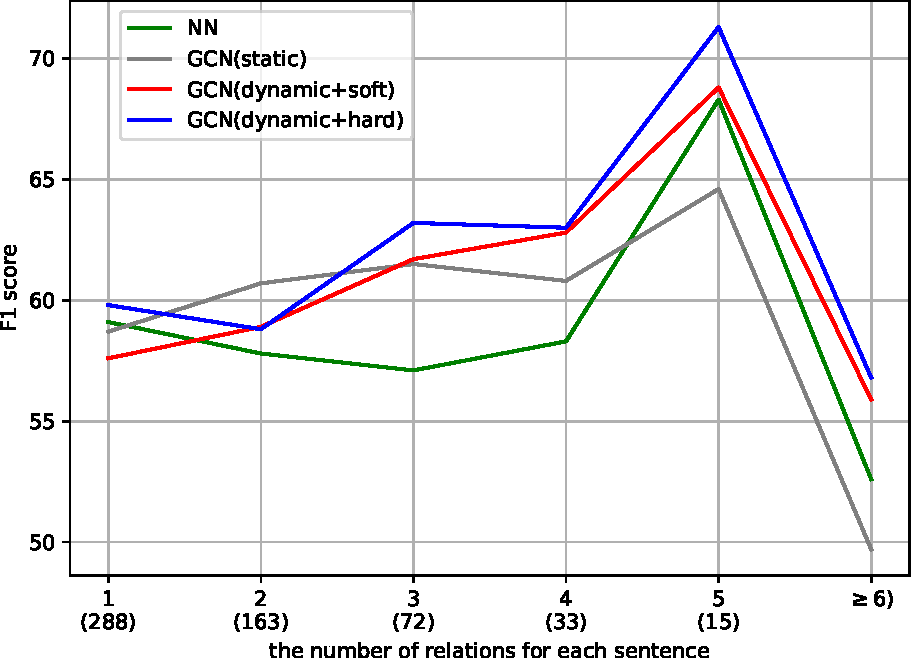
\includegraphics[width=2.8in]{../images/fig-rel-num.pdf}
    \end{center}
   \caption{F1 scores with respect to the number of relations for each sentence.
    The numbers in parentheses are counts of sentences in the ACE05 test set.}
    \label{fig:rel_num}
\end{figure}


%\begin{figure}
%    \begin{center}
%        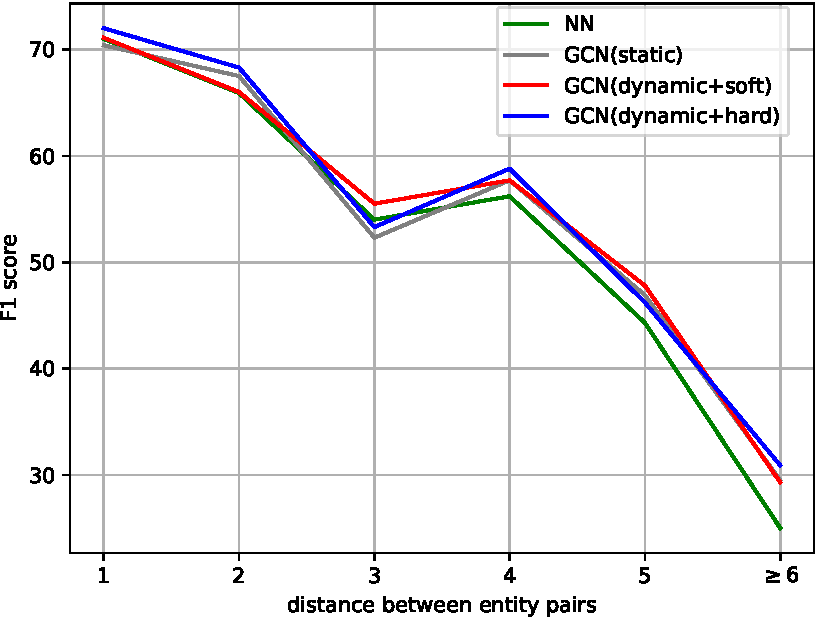
\includegraphics[width=3.0in]{../images/fig-distance.pdf}
%    \end{center}
%     \caption{F1 scores on ACE05 dataset with respect to the distance between entity pairs.}
%    \label{fig:len}
%\end{figure}


%Fifthly,
%we analysis the relation performance with respect to
%different distances between entity pairs (Figure \ref{fig:len}).
%Our GCN-based models achieve better performance for larger distance ($>3$).
%It shows that the GCN could capture some long distance dependency
%for joint extraction task.
%In addition,
%all models are not good at extracting relations over very long distances.
%Thus,  combining joint decoding algorithms
%with our model might be a promising direction in this joint extraction task.


Finally,
We compare the ``NN'' model with the ``GCN'' model
on some concrete examples, as shown in Table \ref{tab:case}.
For S1,
the ``NN'' wrongly identifies the relation \texttt{GEN-AFF} between 
``[legislature]\textsuperscript{\texttt{ORG}}'' and
``[north korea]\textsuperscript{\texttt{GPE}}''
even though the relation $\texttt{ORG-AFF}$ between 
``[legislature]\textsuperscript{\texttt{ORG}}'' and
``[chairman]\textsuperscript{\texttt{PER}}'' is detected.
For S2,
the ``NN'' does not detect \texttt{PART-WHOLE} relation 
while the ``GCN'' correctly find it.
These two observations show that our ``GCN'' is good at 
dealing with the situation 
when the multiple relations share common entities, as expected.
For S3,
our ``GCN'' identifies a \texttt{PHYS} relation between
``[units]\textsuperscript{\texttt{PER}}'' and
``[captial]\textsuperscript{\texttt{GPE}}'',
while the ``NN'' does not find this relation 
even the entities are correct.
However, both models do not identify the relation \texttt{ART} between
``[units]\textsuperscript{\texttt{PER}}'' and
``[weapons]\textsuperscript{\texttt{WEA}}''.
We think advanced improvement methods
which use more powerful graph neural network might be helpful
in this situation.


\subsection{Golden Entity Results on ACE05}
\begin{table}
	\centering
	\footnotesize
	\begin{tabular}{l|lll}
		\toprule
		\textbf{Model} & \multicolumn{3}{c}{\textbf{Relation}} \\
        \midrule
        M\&B \citeyearpar{miwa-bansal:2016:P16-1}  & \textbf{70.1} & 61.2 & 65.3  \\
        C\&M \citeyearpar{P18-2014} & 69.7 & 59.5 & 64.2 \\
        NN & 68.5 & 62.8 & 65.5 \\
     
        GCN (static) & 69.1 & 63.8 & 66.4 \\
        GCN (dynamic + soft)& 68.7 & 63.4 & 65.9 \\
        GCN (dynamic + hard)& 68.7 & \textbf{65.4} & \textbf{67.0}  \\
		\bottomrule
	\end{tabular}
	\caption{\small Results on the ACE05 dataset with golden entity.}
	\label{tab:ace-gold-entity}
\end{table}


In order to compare with relation classification methods,
we evaluate our models with golden entities on ACE05 corpus in Table \ref{tab:ace-gold-entity}.
We use the same data split to compare with their model \cite{miwa-bansal:2016:P16-1,P18-2014}.
We do not tune hyperparameters extensively. 
For example, we use the same setting in both end-to-end and golden entity
rather than tune parameters on each of them.
The baseline systems are \cite{miwa-bansal:2016:P16-1} and \cite{P18-2014}.

In general, 
our ``NN''  is competitive,
comparing to the dependency tree-based state-of-the-art model \cite{miwa-bansal:2016:P16-1}.
It shows that our CNN-based neural networks are able to extract
more powerful features to help relation extraction task.
After adding GCN,
our GCN-based models achieve the better performance.
This indicates that the proposed models can
achieve large improvement without any external syntactic tools
\footnote{For simplicity, we do not extract golden entity type features explicitly in our model.
And we believe there will be further improvements when these features are used.
}.

\begin{table*}
    \centering
    \renewcommand{\multirowsetup}{\centering}  
    \label{tab:err-1}
    % \vspace{0.2cm}
    \begin{tabular}{p{0.06\linewidth}|p{0.9\linewidth}}
        \toprule
        S1 & % however the firm announced on friday that it had reached a deal with 
        the 
        $\text{[british]}_{\texttt{GEN-AFF-2}: \heartsuit \clubsuit  \spadesuit}^{\texttt{GPE}:\heartsuit \clubsuit \spadesuit}$
        $\text{[arm]}_{\texttt{PART-WHOLE-1}: \heartsuit \spadesuit | \texttt{GEN-AFF-1}: \heartsuit \clubsuit \spadesuit}^{\texttt{ORG}:\heartsuit \clubsuit \spadesuit}$
        of french distributors 
        $\text{[pathe]}_{\texttt{PART-WHOLE-2}: \heartsuit \spadesuit}^{\texttt{ORG}:\heartsuit \clubsuit \spadesuit}$
        to show four releases . 
        \\
        \bottomrule
    \end{tabular}
    
    \label{tab:err-2}
    % \vspace{0.2cm}
    \begin{tabular}{p{0.06\linewidth}|p{0.9\linewidth}}
        \toprule
        S2 &
        %during their visit to pyongyang , weldon 's delegation also met choe thae bok , 
        \dots
        $\text{[chairman]}_{\texttt{ORG-AFF-1}: \heartsuit \clubsuit \spadesuit}^{\texttt{PER}:\heartsuit \clubsuit \spadesuit}$
        of 
        $\text{[north korea ]}_{\texttt{PART-WHOLE-2}: \heartsuit \spadesuit | \texttt{GEN-AFF-2}: \clubsuit}^{\texttt{GPE}:\heartsuit \clubsuit \spadesuit}$
        's 
        $\text{[legislature]}_{\texttt{PART-WHOLE-1}: \heartsuit \spadesuit| \texttt{ORG-AFF-2}: \heartsuit \clubsuit \spadesuit | \texttt{GEN-AFF-1}: \clubsuit}^{\texttt{ORG}:\heartsuit \clubsuit \spadesuit}$
        , the supreme people  's assembly .    
        \\
        \bottomrule
    \end{tabular}
    \label{tab:err-3}
    \begin{tabular}{p{0.06\linewidth}|p{0.9\linewidth}}
        \toprule
        S3 & 
         % u.s. officials say some intelligence indicates 
         a red line may have been drawn around the 
        $\text{[capital]}_{\texttt{PHYS-2}: \heartsuit \spadesuit}^{\texttt{GPE}:\heartsuit \clubsuit \spadesuit}$ 
        with 
        $\text{[republican gurad]}_{\texttt{ORG-AFF-2}: \heartsuit \clubsuit \spadesuit}^{\texttt{ORG}:\heartsuit \clubsuit \spadesuit} $
        $\text{[units]}_{\texttt{PHYS-1}: \heartsuit \spadesuit| \texttt{ORG-AFF-1}: \heartsuit \clubsuit \spadesuit| \texttt{ART-1}: \heartsuit}^{\texttt{PER}:\heartsuit \clubsuit \spadesuit} $
        ordered to use chemical 
        $\text{[weapons]}_{\texttt{ART-2}: \heartsuit}^{\texttt{WEA}:\heartsuit \clubsuit \spadesuit} $
        once u.s. and allied troops cross it .
        \\
        \bottomrule
    \end{tabular}
    \caption{Examples from the ACE05 dataset
    with label annotations from ``NN'' model and ``GCN'' model
    for comparison. 
    The $\heartsuit$ is the gold standard,
    and the $\clubsuit$, $\spadesuit$ are the output of the ``NN'' 
    ,``GCN'' model respectively.}
    \label{tab:case}
\end{table*}



\section{Related Work}
%\subsection*{Entity Relation Extraction}
There have been extensive studies for entity relation extraction task.
Early work employs a pipeline of methods that extracts entities first,
and then determines their relations \citep{zelenko2003kernel,miwa-EtAl:2009:EMNLP,chan-roth:2011:ACL-HLT2011,lin-EtAl:2016:P16-1}.
As pipeline approaches suffer from error propagation, 
researchers have proposed methods for joint entity relation extraction.

Parameter sharing is a basic strategy for joint extraction.
For example,
\citet{miwa-bansal:2016:P16-1} propose a neural method comprised of 
a sentence-level RNN for extracting entities,
and a dependency tree-based RNN to predict relations.
Their relation model takes hidden states of the entity model as features
(i.e., the shared parameters).
Similarly,
\citet{katiyar-cardie:2017:Long} use a simplified relation model
based on the entity RNN using the attention mechanism.
These joint methods do joint learning through sharing parameters and they have no explicit interaction in type inference. 

To further explore interactions between the entity decoder
and the relation decoder,
many of them focus on some joint decoding algorithms.
ILP-based joint decoder \cite{yang2013joint},
CRF-based joint decoder \cite{katiyar-cardie:2016:P16-1},
joint sequence labelling tag set \cite{zheng-EtAl:2017:Long},
beam search \cite{li-ji:2014:P14-1},
global normalization \cite{zhang-zhang-fu:2017:EMNLP2017},
and transition system \cite{wang2018joint} are investigated.
%One similar network structure to our model is proposed in
%\cite{D18-1249}.
%They jointly extract entities and relations using
%``RNN + CNN'' network structure.
Different from models there, we propose a novel and concise
joint model to handle joint type inference based on 
graph convolutional networks,
which can capture information between multiple entity types 
and relation types explicitly\footnote{In addition, 
transfer learning\cite{sun2019distantly}, multi-task learning \cite{sanh2018hierarchical} for this task were also studied.
In order to make a fair comparison,
we do not include these models in experiments.}.



%\subsection*{Graph Neural Networks}
Recently,
researches of graph neural networks (GNNs) have been receiving more and more attention 
because of the great expressive power of graphs \cite{cai2018comprehensive,battaglia2018relational,zhou2018graph}.
Graph Convolutional Network (GCN) is one of the typical variants of GNN
\cite{bruna2013spectral,defferrard2016convolutional,kipf2017semi}.
It has been successfully applied to many NLP tasks
such as text classification \cite{yao2018graph},
semantic role labeling \cite{marcheggiani2017encoding},
relation extraction \cite{zhang2018graph}
machine translation \cite{bastings2017graph} and
knowledge base completion \cite{shang2018end}.
We note that most previous applications of GCN focus on a single job,
while the joint entity relation extraction consists of multiple sub-tasks.
Investigating GCN in joint learning scenarios is the main topic of this work.
A closely related work is \cite{P18-2014}, which focuses on relation extraction with golden entities.
Our work can be viewed as an end-to-end extension of their work.








\section{Conclusion}
We propose a novel and concise joint model
based on GCN
to perform joint type inference
for entity relation extraction task.
Compared with existing joint methods,
it provides a new way to 
capture the interactions on multiple entity types and relation types explicitly in a sentence.
%By introducing a binary relation classification task,
%our method could utilize the structure of entity-relation bipartite graph in a more efficient and interpretable way.
Experiments on ACE05
dataset show the effectiveness of the proposed method.

\section*{Acknowledgement}

The authors wish to thank the reviewers for their helpful
comments and suggestions.
This research is (partially) supported by
STCSM (18ZR1411500), NSFC(61673179) and the Foundation of State Key Laboratory of Cognitive Intelligence, iFLYTEK(COGOS-20190003).
The corresponding authors are Yuanbin Wu and Shiliang Sun.

\bibliography{acl2019}
\bibliographystyle{acl_natbib}

\end{document}
